\documentclass{InsightArticle}
\usepackage[dvips,
bookmarks,
bookmarksopen,
backref,
colorlinks,linkcolor={blue},citecolor={blue},urlcolor={blue},
]{hyperref}
\usepackage{listings}


\title{Binary morphological closing and opening image filters}
\release{1}
\author{Ga\"etan Lehmann}
\authoraddress{Biologie du d\'eveloppement et de la reproduction, INRA de Jouy-en-Josas}


\begin{document}
\lstset{language=c++}
\maketitle

\ifhtml
\chapter*{Front Matter\label{front}}
\fi


\begin{abstract}
\noindent
Binary morphological closing and opening image filters remove structures smaller than the structuring element in a binary image.
\end{abstract}
% \keyword{mathematical morphology, binary image, opening, closing}

\tableofcontents


\section{Description}

Binary morphological closing and opening image filters remove structures smaller than the structuring element in a binary image. These filters suppress the boundary effects and maintain the background values.

\section{Implementation}

BinaryMorphologicalClosingImageFilter and BinaryMorphologicalOpeningImageFilter are mainly a sequence of filters.

BinaryMorphologicalOpeningImageFilter runs a BinaryErodeImageFilter followed by a BinaryDilateImageFilter. Some background pixels may appear in the output image therefore the user can choose the value of added background pixels.

BinaryMorphologicalClosingImageFilter runs a BinaryDilateImageFilter followed by a BinaryErodeImageFilter\footnote{BinaryMorphologicalClosingImageFilter and BinaryMorphologicalOpeningImageFilter use intensively BinaryDilateImageFilter and BinaryErodeImageFilter, but a bug occures in these filters when the requested region is smaller than the available one. A version of these filters which fixes that bug can be found in the archive. More details at http://public.kitware.com/pipermail/insight-users/2005-September/014844.html.}. If SafeBorder is true (setting by default), the BinaryDilateImageFilter is preceded by a ConstantPadImageFilter and the BinaryErodeImageFilter is followed by a CropImageFilter in order to avoid border effects. Finally, BinaryMorphologicalClosingImageFilter copy the background pixels from the input image to avoid the modifications of the background done by the BinaryErodeImageFilter. BinaryMorphologicalClosingImageFilter will never add background pixels so the background value used for the BinaryErodeImageFilter is automatically chosen.

\section{Usage}

First of all, the user must create a structuring element. As usual, the headers must be included

\begin{lstlisting}
#include "itkBinaryBallStructuringElement.h"
#include "itkBinaryMorphologicalOpeningImageFilter.h"
#include "itkBinaryMorphologicalClosingImageFilter.h"
\end{lstlisting}
Create the structuring element - a disk of radius 40
\begin{lstlisting}
typedef itk::BinaryBallStructuringElement
  < PType, dim> KernelType;
KernelType ball;
KernelType::SizeType ballSize;
ballSize.Fill( 40 );
ball.SetRadius(ballSize);
ball.CreateStructuringElement();
\end{lstlisting}
Create the closing filter
\begin{lstlisting}
typedef itk::BinaryMorphologicalClosingImageFilter
  < IType, IType, KernelType > CloseType;
CloseType::Pointer close = CloseType::New();
close->SetInput( filter->GetOutput() );
close->SetKernel( ball );
\end{lstlisting}
The SetSafeBorder() method can be used to disable the safe border option (see Figure~~\ref{unsafe})
\begin{lstlisting}
close->SetSafeBorder( false );
\end{lstlisting}
The SetForegroundValue() can be used to set the foreground value used for the closing. The default is itk::NumericTraits$<$ PType $>$::max()
\begin{lstlisting}
close->SetForegroundValue( 200 );
\end{lstlisting}
Create the opening filter
\begin{lstlisting}
typedef itk::BinaryMorphologicalOpeningImageFilter
  < IType, IType, KernelType > OpenType;
OpenType::Pointer erode = OpenType::New();
erode->SetInput( filter->GetOutput() );
erode->SetKernel( ball );
\end{lstlisting}
The SetForegroundValue() can be used to set the foreground value used for the opening. The default is itk::NumericTraits$<$ PType $>$::max()
\begin{lstlisting}
erode->SetForegroundValue( 200 );
\end{lstlisting}
The SetBackgroundValue() method can be used to set the value of pixels which will be moved to backgound (see Figure\ref{open}). The default is itk::NumericTraits$<$ PType $>$::Zero
\begin{lstlisting}
erode->SetBackgroundValue( 150 );
\end{lstlisting}

\section{Examples}

\begin{figure}[b]
\centering
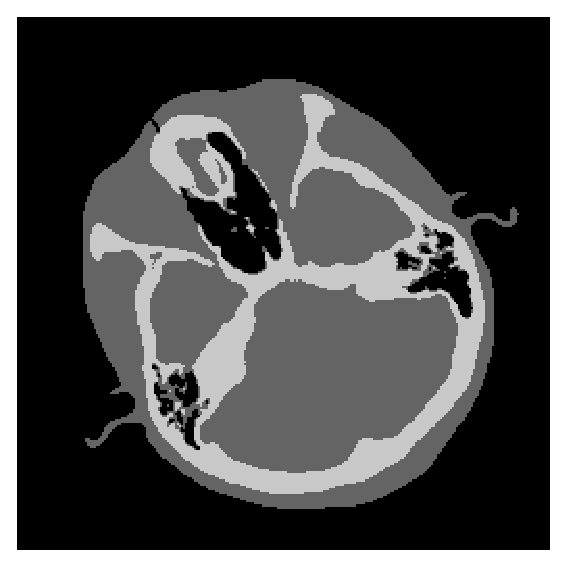
\includegraphics{2th_cthead1.eps}
\caption{The input image. The image contains 3 pixels values: black (0), dark grey (100) and light grey (200). Each those values can be used as foreground value. In the next examples, the light grey is used as foreground and the other values as background.}
\end{figure}

\begin{figure}
\centering
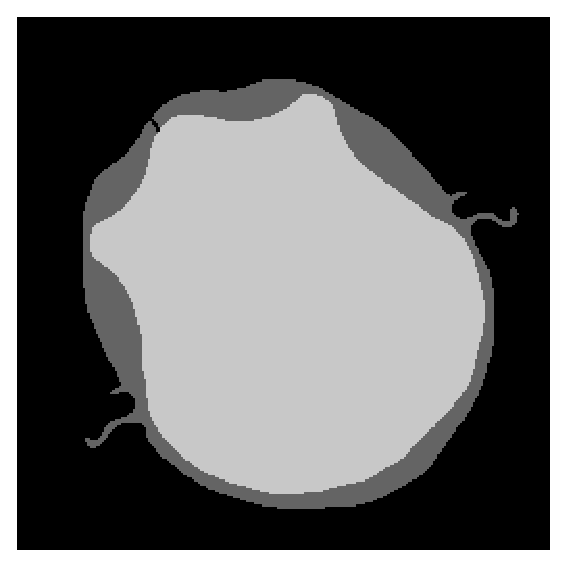
\includegraphics{close.eps}
\caption{The input image closed by a disc of radius 40, with SafeBorder=true. All background regions smaller than the structuring element are filled with the foreground value. The other background regions are not modified.}
\end{figure}

\begin{figure}
\centering

\includegraphics{close-unsafe.eps}
\caption{The input image closed by a disc of radius 40, with SafeBorder=false. The border effects are clearly visible on the right and bottom side of the image, but are also there on the top and left side of the image. SafeBorder=false must be used very carefully.\label{unsafe}}
\end{figure}

\begin{figure}
\centering
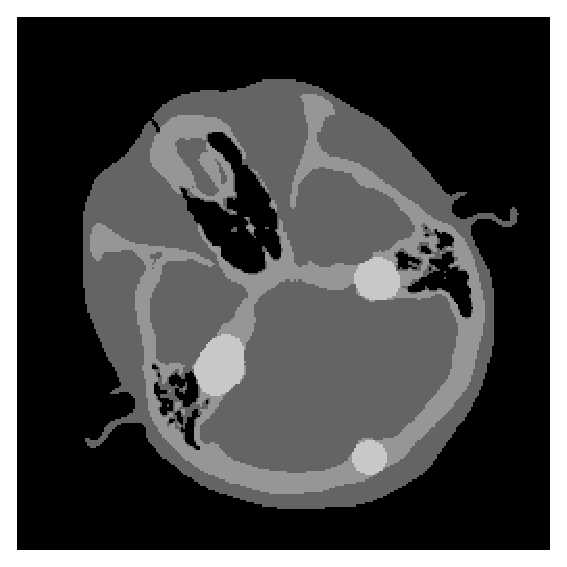
\includegraphics{open.eps}
\caption{The opened image with a disc of radius 8. Only the foreground (light grey) regions of the input image where the structuring element fit are kept in light grey; the other foreground regions are added to the background (in-between grey (150)).\label{open}}
\end{figure}

\end{document}
